\documentclass[11pt,a4paper]{article}
\usepackage[utf8x]{inputenc}
\usepackage[T1]{fontenc}
%\usepackage{gentium}
\usepackage{mathptmx} % Use Times Font

\usepackage{graphicx} % Required for including pictures
\usepackage{hyperref} % Format links for pdf
\usepackage[british]{babel} % Multilingual bibliographies
\usepackage{natbib}
\setlength{\bibsep}{0.0pt}

\frenchspacing % No double spacing between sentences
\usepackage[margin=1in]{geometry}

\usepackage[all]{nowidow} % Tries to remove widows
\usepackage[protrusion=true,expansion=true]{microtype} % Improves typography, load after fontpackage is selected

\usepackage{lipsum} % Used for inserting dummy 'Lorem ipsum' text into the template

\title{My datascience project title}
\author{Irma Student and Soham Eye}
%\usepackage{natbib}

\begin{document}

\maketitle

%% INSTRUCTIONS:
%%
%% 1. Please rename this file fds-project-option-1.tex,
%% fds-project-option-2.tex, or fds-project-option-3.tex, depending on
%% which project option you are doing. When you submit, please submit
%% the PDF file with the corresponding name.
%% 
%% 2. You can edit either using:
%%
%%    a. Overleaf professional, a collabaratorive LaTeX editor. See
%%       https://www.overleaf.com/edu/edinburgh for documentation. Create an
%%       empty document, and copy the files in this directory to it.
%%
%%    b. A LaTeX editor on your PC - you can commit changes to this
%%       repository to collaborate.
%% 
%% 3. Please keep the section and paragraph headings as they are.
%%
%% 4. The word limit for the Overview section is mandatory. For the
%% other sections word limits are suggested.
%%
%% 5. The page limits must be strictkly adhered to, and depend on if
%% you are working individually, in pairs or in threes:
%%
%%   - Individual: 6 pages 
%%   - Pairs: 8 pages 
%%   - Threes: 10 pages 
%%

\section{Overview}
% 250 words maximum

\section{Introduction}
% Suggested 400 words

\paragraph{Context and motivation}

What is the area of this data science study, and why is it interesting
to investigate?

\paragraph{Previous work}

Brief description of any previous work in this area (e.g., in the
media, or scientific literature or blogs).

E.g. Recent surveys show that most students prefer final projects to
final exams \cite{Space2021}. 

\paragraph{Objectives}

What questions are you setting out to answer?

\section{Data}
% Suggested 300 words

\paragraph{Data provenance} Who created the dataset(s)?  How you have
obtained it (e.g., file or web scraping), and do the T\&Cs allow you
to use obtain the data for the project?

\paragraph{Data description} Description of the data, e.g. variables
in each table, number of records.

\paragraph{Data processing} How you have processed the dataset, e.g.,
cleaning, removing missing values, joining tables.

\section{Exploration and  analysis}
% Suggested 500 words for individual report; proportionately longer
% for group projects).

% 't' means "try to position at the top of the page"
\begin{figure}[t]
  \centering
  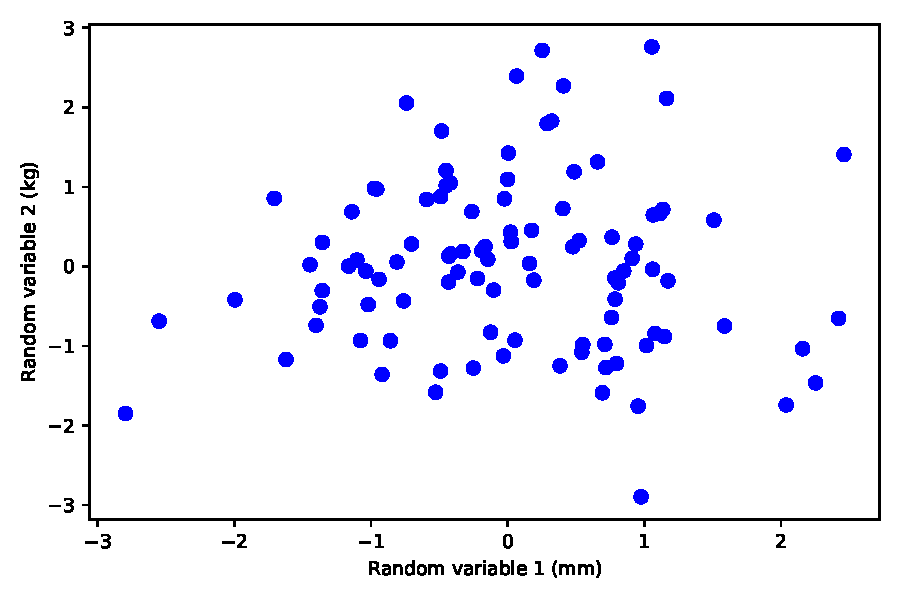
\includegraphics{example1}
  \caption{Demonstration figure. This caption explains more about the
    figure. Note that the font size of the labels in the plot is 9pt,
    which is obtained by the settings as shown in the Jupyter
    notebook.}
  \label{fds-project-template:fig:example1}
\end{figure}

% 'b' means "try to position at the bottom of the page"
\begin{table}[b]
  \caption{Exerpt from Scottish Index of Multiple Deprivation, 2016 edition.
    \url{https://simd.scot}. You may put more information in the caption.}
  \label{tab:example1}
\begin{tabular}{lrrrrrrr}
\hline\hline
\textbf{Location}&\textbf{Employ-}&\textbf{Illness}&\textbf{Attain-}&\textbf{Drive}  &\textbf{Drive}    &\textbf{Crime}&\dots\\
                 &\textbf{ment}   &                &\textbf{ment}   &\textbf{Primary}&\textbf{Secondary}&              &\\
\hline
\textbf{Macduff}&$10$&$ 95$&$5.3$&$1.5$&$6.6$&$249$&\dots\tabularnewline
\textbf{Kemnay}&$ 3$&$ 40$&$5.3$&$2.4$&$2.4$&$168$&\dots\tabularnewline
\textbf{Hilton}&$ 0$&$ 10$&$6.3$&$2.2$&$3.0$&$144$&\dots\tabularnewline
\textbf{Ruchill}&$ 8$&$130$&$4.9$&$1.7$&$5.6$&$318$&\dots\tabularnewline
\textbf{Belmont}&$ 2$&$ 50$&$6.1$&$3.1$&$3.2$&$129$&\dots\tabularnewline
\dots&\dots&\dots&\dots&\dots&\dots&\dots&\dots\tabularnewline
\hline
\end{tabular}
\end{table}

A data science analysis of the paper, including: 
\begin{itemize}
\item Visualisations (for example
  Figure~\ref{fds-project-template:fig:example1}) and tables (for
  example Table~\ref{tab:example1}). Please make sure that all figures
  and tables are referred to in the text, as demonstrated in this
  bullet point.
\item Interpretation of the results 
\item Description of how you have applied one ore more of the
  statistical and ML methods learned in the FDS to the data
\item Interpretation of the findings 
\end{itemize}

You can use equations like this:
\begin{equation}
  \label{fds-project-template:eq:1}
  \overline{x} = \sum_{i=1}^n x_i
\end{equation}
or maths inline: $E=mc^2$. However, you do not need to reexplain techniques that you have learned in the course -- assume the reader undertands linear regression, logicstic regression K-nerest neighbours etc.  Remember to explain any symbols use, e.g.~``$n$ is the number of data points and $x_i$ is the value of the $i$th data point.''.

\section{Discussion and conclusions}
% Suggested 400 words.

\paragraph{Summary of findings}

\paragraph{Evaluation of own work: strengths and limitations}

\paragraph{Comparison with any other related work}
E.g. ``Anscombe has also demonstrated that many patterns of data can
have the same correlation coefficient'' \cite{Ansc73Grap}.

\paragraph{Improvements and extensions}

\bibliographystyle{unsrt}
\bibliography{fds-project}
\end{document}
